\section{Python Sample applications}
\label{sec:PythonSampleApps}

The first two examples in this section are simple applications developed in COMPSs to easily illustrate how to code,
compile and run COMPSs applications. These applications are executed locally and show different ways to take advantage
of all the COMPSs features. 

The rest of the examples are more elaborated and consider the execution in a cloud platform where the VMs mount a common 
storage on \textbf{/sharedDisk} directory. This is useful in the case of applications that require working 
with big files, allowing to transfer data only once, at the beginning of the execution, and to enable 
the application to access the data directly during the rest of the execution.

The Virtual Machine available at our webpage (\url{http://compss.bsc.es/}) provides a development environment with
all the applications listed in the following sections. The codes of all the applications can be found under the 
$/home/compss/workspace\_python/$ folder. 

%%%%%%%%%%%%%%%
%% SIMPLE
%%%%%%%%%%%%%%%
\subsection{Simple}
The Simple application is a Python application that increases a counter by means of a task. The counter is stored inside a file that 
is transfered to the worker when the task is executed. Next, we provide the main code and the task declaration:

\begin{lstlisting}[language=python]
def main_program():
    from pycompss.api.api import compss_open

    # Check and get parameters
    if len(sys.argv) != 2:
        usage()
        exit(-1)
    initialValue = sys.argv[1]
    fileName="counter"

    # Write value
    fos = open(fileName, 'w')
    fos.write(initialValue)
    fos.close()
    print "Initial counter value is " + initialValue

    # Execute increment
    increment(fileName)

    # Write new value
    fis = compss_open(fileName, 'r+')
    finalValue = fis.read()
    fis.close()
    print "Final counter value is " + finalValue
\end{lstlisting}

\begin{lstlisting}[language=python]
@task(filePath = FILE_INOUT)
def increment(filePath):
    # Read value
    fis = open(filePath, 'r')
    value = fis.read()
    fis.close()

    # Write value
    fos = open(filePath, 'w')
    fos.write(str(int(value) + 1))
    fos.close()
\end{lstlisting}

The simple application can be executed by invoking the runcompss command with the \textit{--lang=python} flag. The following lines provide
an example of its execution.

\begin{lstlisting}[language=bash]
compss@bsc:~$ cd ~/workspace_python/simple/
compss@bsc:~/workspace_python/simple$ runcompss --lang=python ~/workspace_python/simple/simple.py 1
Using default location for project file: /opt/COMPSs/Runtime/configuration/xml/projects/project.xml
Using default location for resources file: /opt/COMPSs/Runtime/configuration/xml/resources/resources.xml

----------------- Executing simple.py --------------------------

WARNING: IT Properties file is null. Setting default values
[   API]  -  Deploying COMPSs Runtime v<version>
[   API]  -  Starting COMPSs Runtime v<version>
Initial counter value is 1
Final counter value is 2
[   API]  -  No more tasks for app 0
[   API]  -  Getting Result Files 0
[   API]  -  Execution Finished

------------------------------------------------------------
\end{lstlisting}

%%%%%%%%%%%%%%%
%% INCREMENT
%%%%%%%%%%%%%%%
\subsection{Increment}
The Increment application is a Python application that increases N times three different counters. Each increase step is developed by a separated task. The
purpose of this application is to show parallelism between the three counters.

Next we provide the main code of this application. The code inside the \textit{increment} task is the same than the previous example. 

\begin{lstlisting}[language=python]
 def main_program():
    # Check and get parameters
    if len(sys.argv) != 5:
        usage()
        exit(-1)
    N = int(sys.argv[1])
    counter1 = int(sys.argv[2])
    counter2 = int(sys.argv[3])
    counter3 = int(sys.argv[4])

    # Initialize counter files
    initializeCounters(counter1, counter2, counter3)
    print "Initial counter values:"
    printCounterValues()

    # Execute increment
    for i in range(N):
        increment(FILENAME1)
        increment(FILENAME2)
        increment(FILENAME3)

    # Write final counters state (sync)
    print "Final counter values:"
    printCounterValues()
\end{lstlisting}

As shown in the main code, this application has 4 parameters that stand for:

\begin{enumerate}
 \item \textbf{N:} Number of times to increase a counter
 \item \textbf{counter1:} Initial value for counter 1
 \item \textbf{counter2:} Initial value for counter 2
 \item \textbf{counter3:} Initial value for counter 3
\end{enumerate}

Next we run the Increment application with the \textit{-g} option to be able to generate the final graph at the end of the execution.

\begin{lstlisting}[language=bash]
compss@bsc:~/workspace_python/increment$ runcompss --lang=python -g ~/workspace_python/increment/increment.py 10 1 2 3
Using default location for project file: /opt/COMPSs/Runtime/scripts/configuration/xml/projects/project.xml
Using default location for resources file: /opt/COMPSs/Runtime/scripts/configuration/xml/resources/resources.xml

----------------- Executing increment.py --------------------------

WARNING: IT Properties file is null. Setting default values
[   API]  -  Deploying COMPSs Runtime v<version>
[   API]  -  Starting COMPSs Runtime v<version>
Initial counter values:
- Counter1 value is 1
- Counter1 value is 2
- Counter1 value is 3
Final counter values:
- Counter1 value is 11
- Counter1 value is 12
- Counter1 value is 13
[   API]  -  No more tasks for app 0
[   API]  -  Getting Result Files 0
[   API]  -  Execution Finished

------------------------------------------------------------
\end{lstlisting}

By running the \textit{gengraph} command users can obtain the task graph of the above execution. Next we provide the set of commands
to obtain the graph show in Figure \ref{fig:increment_python}.

\begin{lstlisting}[language=bash]
compss@bsc:~$ cd ~/.COMPSs/increment.py_01/monitor/
compss@bsc:~/.COMPSs/increment.py_01/monitor$ gengraph complete_graph.dot
compss@bsc:~/.COMPSs/increment.py_01/monitor$ evince complete_graph.pdf
\end{lstlisting}

\begin{figure}[ht!]
  \centering
    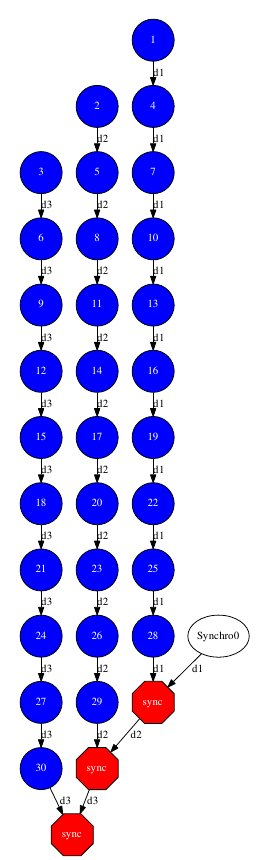
\includegraphics[width=0.3\textwidth]{./Sections/3_Python/Figures/increment_graph.jpeg}
    \caption{Python increment tasks graph} 
    \label{fig:increment_python}
\end{figure}

%%%%%%%%%%%%%%%
%% WORDCOUNT
%%%%%%%%%%%%%%%
\newpage
%\subsection{WordCount}


%%%%%%%%%%%%%%%
%% MATMUL
%%%%%%%%%%%%%%%
%\subsection{Matmul}

%%%%%%%%%%%%%%%
%% NEURONS
%%%%%%%%%%%%%%%
%\subsection{Neurons}
